\documentclass{subfiles}

\begin{document}
	
	\par As mentioned at Section \ref{sec:Problem}, there are very few uses of FW LiDAR data because of the quantity of the recorded information. For that reason, DASOS was developed DASOS (Section \ref{DASOS}), as an open source software, to help foresters without computer science background to use FW LiDAR data. In this section:
	
	\begin{itemize}
		\item An overview of related software packages is given and we explain how DASOS differs from those packages (Section \ref{LiDARsoftwares}).
		\item  The main method of interpreting the data within DASOS (the voxelisation approach) is described (Subsection \ref{Voxelisation}).
		\item Then all the functionalities of DASOS are listed (Section \ref{DASOS})
		\item and finally a summary is provided (Section \ref{DASOS-Vol-Summary}).
	\end{itemize}
	
	
	\section{State-of-Art FW LiDAR Software Packages}\label{LiDARsoftwares}
	
	\par {\color{blue}The most common approach of interpreting the FW LiDAR is the Gaussian decomposition of the waveforms for peak points extraction. Each waveform is modelled as a set of Gaussian pulses and for every Guassian peak, a discrete LiDAR point is extracted} ~\cite{Wanger2006}. Neunschwander et al used this approach for Landcover classification ~\cite{Neuenschwander2009} while Reitberger et al applied it for distinguishing deciduous trees from coniferous trees ~\cite{Reitberger2008}. Chauve et al further proposed an approach of improving the Gaussian model in order to increase the density of the points extracted from the data and consequently improve point based classifications of FW LiDAR data ~\cite{Chauve2007}.  The following tools are able to extract discrete points from the waveforms and visualise small areas of interest:
	 
	\begin{itemize}
		\item \textbf{Pulsewaves}: visualise a small number of waveforms using different transparencies according to the intensities of the wave-samples and are able to generate discrete point clouds \cite{Isenburg2012Pulsewaves}. \newline Link: \url{<https://rapidlasso.com/pulsewaves/>}
	    \item \textbf{FullAnalyze}: supports echo decomposition. Regarding visualisations the user can select single trees from the Graphical User Interface (GUI) and for each wave-sample, a sphere with radius proportional to its amplitude is created and visualised \cite{Chauve2009}. \newline Link: \url{<http://fullanalyze.sourceforge.net/>} 
    	\item \textbf{SPDlib}: exports discrete LiDAR and visualises either the samples that are above a threshold level as points or the extracted discrete point cloud. It also colours them according to their intensity value\cite{Bunting2013}. \newline Link: \url{<http://www.spdlib.org/>} 
	\end{itemize}

	\par  Echo decomposition and extraction of peak points identifies significant features and further enables the interpretation of the data within existing workflows and software that support discrete LiDAR data. For example, the discrete LiDAR can be analysed using: 
	
	\begin{itemize}
	\item \textbf{Lag}: a visualisation tool for analysing and inspecting discrete LiDAR point clouds. \newline Link: \url{<http://arsf.github.io/lag/>}
	
	\item \textbf{Quick Terrain Modeller} : a 3D discrete LiDAR points visualiser, that can generate Digital Elevation Models (DEM) and Digital Terrain Models (DTM). \newline Link: \url{<http://appliedimagery.com/>}
	
	\item \textbf{LAStools} : a tool set that classifies noise, visualises point clouds, clips data.  \newline Link \url
	\end{itemize}
		
	\par DASOS approach of interpreting FW LiDAR data is fundamentally different from the aforementioned software packages. On the one hand, converting FW LiDAR into discrete, their usage is ease since existing overflows support discrete LiDAR, but on the other hand FW LiDAR contain information about pulse width that are not preserved after peak point extraction. Also the comparison of point clouds depends on the density of the emitted pulses; problems arise with the sinusoidal pattern of the Leica system. For that reason, in DASOS, this information is accumulated from multiple shots into a voxel array, building up a 3D density volume. The correlation between multiple pulses in a voxel representation produces a more accurate and complete representation, which confers greater noise resistance and it further opens up possibilities of vertical interpretation of the data. The idea of voxelising FW LiDAR data is explained in the following section \ref{Voxelisation}.  
	
		
	 \section{Voxelisation for Interpreting FW LiDAR data}\label{Voxelisation}
		
	\par Voxelisation of FW LiDAR data was firstly introduced by Persson et al., who used it to visualise waveforms using different transparencies \cite{Persson2005} and {\color {blue} it has been adopted as the future of FW LiDAR data with the literature moving toward that direction.} In 2016, Cao et al used it for tree species identification \cite{Cao2016} and Sunmall et al characterised forest canopy from a voxelised vertical profile \cite{Sumnall2016}. {\color{blue}The innovative approach of voxelising the FW LiDAR data }is an integral part of this thesis and it is used for both visualisations and classifications \cite{Miltiadou2014}\cite{Miltiadou2015}. 

		
		
	\par The FW LiDAR data are voxelised by inserting the wave samples into a 3D regular grid and constructing a 3D discrete density volume. According to Persson et al, each wave sample is associated with the 3D cell, named voxel, that it lies inside. If multiple samples lie inside a voxel then the sample with the highest intensity is chosen \cite{Persson2005}. In order to reduce noise, there are two differences between this approach and the way FW LiDAR data are voxelised in DASOS. 
		
		
	\par At first a threshold is used to remove low level noise, because when the width of a recorded waveform is longer that the distance between the first hit point and the ground, the system captures low signals, which are pure noise. For that reason, the samples whose intensity is lower than a user-defined noise level/threshold are discarded. 
		
		
		\par Then each wave sample is associated with the voxel that it lies inside and the second difference is how DASOS overcomes the uneven number of samples per voxels. The intensity of each sample is the laser intensity returned during the corresponding time interval. For example, if 5 samples are inside a voxel and the waveform is digitised at 2ns, then the laser intensity associated with that voxel corresponds to a 10ns waveform width. For comparison purposes, it's essential to keep the waveform width consistent across the voxels. For overcoming this issue in DASOS, the average intensity of the samples that lie inside each voxel is taken, instead of choosing the one with the highest intensity \cite{Persson2005}. This way the likelihood of the 3D volume to be affected by outliers and high noise is reduced. The following equation shows how the intensity value of a voxel is calculated:
		
		\begin{eqnarray}
		I_{v} = \dfrac{\sum_{i=1}^{n}I_{i}}{n}
		\end{eqnarray} 
		where 		$I_{v}$ is the accumulated intensity of voxel $v$,
		$n$ is number of samples associated with that voxel and
		$I_{i}$ is the intensity of the sample i.
		
		To sum up, during voxelisation the area of interest is divided into voxels. The samples of the FW LiDAR data are inserted inside this 3D discrete density volume and normalised such that equally sized waveform width is saved inside each voxel. The result is a 3D discrete density volume of the scanned area. Figure \ref{fig:Voxelisation} depicts this process in 2D.
		
		
		\begin{figure} [h!]
			
			
			\begin{subfigure}[t]{.31\textwidth}
				
				\centering
				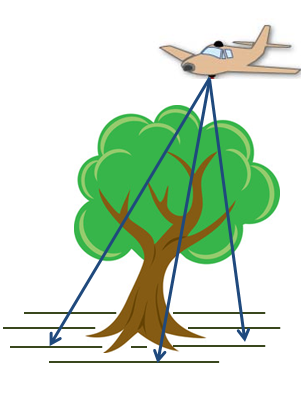
\includegraphics[width=.9\textwidth]{img/VoxelisationA}
				\caption{The sensor from the plane emits multiple pulses and collects information from the returned laser intensity.}
				\label{fig:VoxelisationA_scan}
			\end{subfigure} \hfill
			\begin{subfigure}[t]{.31\textwidth}
				\centering
				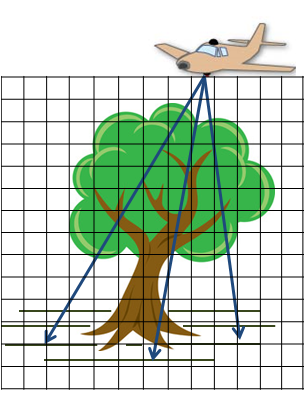
\includegraphics[width=.9\textwidth]{img/VoxelisationB}
				\caption{The area of interest is divided into equally sized cubes, named voxels, generating this way a discrete volume.} 
				\label{fig:VoxelisationB_grid}
			\end{subfigure} \hfill
			\begin{subfigure}[t]{.31\textwidth}
				\centering
				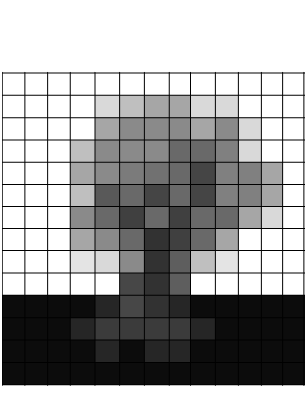
\includegraphics[width=.9\textwidth]{img/VoxelisationC}
				\caption{The accumulated intensities of wave samples into the volume build up the voxelised representation of the scanned area.} 
				\label{fig:VoxelisationC_voxelised}
			\end{subfigure}
			\caption[Voxelisation of FW LiDAR data]{The above images depict the voxelisation process of the FW LiDAR data in 2D. Please note that the voxelisation output in Figure \ref{fig:VoxelisationC_voxelised} shows how ideally the result would look. But in reality, a number of trees may be disconnected from the ground due to missing information about their trunk.} %\footnotemark[1].} 
			\label{fig:Voxelisation} 
		\end{figure}
		
	%	\footnotetext[1]{In Figure \ref{fig:Voxelisation} \newline the tree image is taken from: http://images.clipartpanda.com/tree-clip-artKij4jKriq.jpeg \newline
	%		and the lane image from: http://gmv.cast.uark.edu/wpcontent/uploads/2013/01/ALS\_scematic.jpg  }
	
		
		
	\section{The functionalities of DASOS}\label{DASOS}
	
		\par So far, an overview of existing software packages supporting FW LiDAR was given (Section \ref{LiDARsoftwares}) and it was explained how DASOS differs from them by voxelising the waveforms (Section \ref{Voxelisation}). In this seciton, the three main the functionalities of DASOS are described in table \ref{tbl:functionalities}.
		\newpage
     
        		
        		\begin{longtable}
        			{| p{0.08\linewidth}|p{0.3\linewidth}  | p{0.4\linewidth} | p{0.1\linewidth}|  }
        			\toprule
        			\multicolumn{4}{|c|}{\textbf{1st Functionality: 3D Polygon Mesh Generation }} \\
        			\toprule
        			\textbf{Input}&\textbf{Description} & \textbf{Output Example} & \textbf{Output Format} \\ 
        			\cmidrule(r){1-1}\cmidrule(lr){2-2}\cmidrule(lr){3-3}\cmidrule(l){4-4}
        			LAS1.3& \textbf{3D Polygon Mesh } \newline Constructed from the volumetric representation (algorithms and user-defined parameters are explained in Section \ref{Visualisations} while optimisation approaches are discussed in Section \ref{Optimisations}) \newline & \raisebox{-\totalheight}{\adjincludegraphics[width=\linewidth,trim={0 {0.37\width} 0 0},clip]{img/NewForest}} & .obj \\ 
        			
        			\cmidrule(r){1-1}\cmidrule(lr){2-2}\cmidrule(lr){3-3}\cmidrule(l){4-4}
        			LAS1.3 \newline and \newline level 1 (.bil \& .igm& \textbf{ 3D Coloured \newline Polygon Mesh } \newline Projecting 3 user-defined hyperspectral bands on the mesh (Section \ref{Alignment}) \newline & \raisebox{-\totalheight}{\adjincludegraphics[width=\linewidth,trim={0 0 0 {0.41\width}},clip]{img/NewForest}} & .obj \newline \& \newline .png \\ 
        			
        			\bottomrule
        			
        			\multicolumn{4}{c}{} \\
        			
        			%%
        			\toprule
        			\multicolumn{4}{|c|}{\textbf{2nd Functionality: Generation of 2D metrics}} \\
        			\multicolumn{4}{|c|}{\textbf{aligned with hyperspectral imagery }} \\
        			\toprule

					\multicolumn{4}{|c|}{In Section \ref{Alignment} a selection of the following metrics are used} \\
					\multicolumn{4}{|c|}{for generating tree coverage maps} \\

        				%%
        		
        		
        		
        		        		
        		\toprule
        		\textbf{Input}&\textbf{Metric Description} \newline (L for LiDAR metrics \& H for hyperspectral metrics) & \textbf{Output Example} & \textbf{Output Format} \\ 
        		
        			%%
        		
        		\cmidrule(r){1-1}\cmidrule(lr){2-2}\cmidrule(lr){3-3}\cmidrule(l){4-4}
        		LAS1.3& \textbf{L0 - Height: } \newline The distance between the top non-empty voxel and the lower boundaries of the volume.& \raisebox{-\totalheight}{\adjincludegraphics[width=\linewidth,trim={{.1\width} 0 {.25\width} 0},clip]{img/metrics/HEIGHT}} & .asc \\ 
        		
        		\cmidrule(r){1-1}\cmidrule(lr){2-2}\cmidrule(lr){3-3}\cmidrule(l){4-4}
        		LAS1.3& \textbf{L1 - Thickness: } \newline The distance between  the  first  and  last  non  empty  voxels  in every   column of the   3D   volume.& \raisebox{-\totalheight}{\adjincludegraphics[width=\linewidth,trim={{.1\width} 0 {.25\width} 0},clip]{img/metrics/THICKNESS}} & .asc \\ 
        		
        	
        		
        		\cmidrule(r){1-1}\cmidrule(lr){2-2}\cmidrule(lr){3-3}\cmidrule(l){4-4}				
        		LAS1.3& \textbf{L2 - Density:} \newline Number of non-empty voxel over all voxels within  the  range  from the first to last non-empty voxels. &       \raisebox{-\totalheight}{\adjincludegraphics[width=\linewidth,trim={{.1\width} 0 {.25\width} 0},clip]{img/metrics/DENSITY}} & .asc \\ 
        		
        		\cmidrule(r){1-1}\cmidrule(lr){2-2}\cmidrule(lr){3-3}\cmidrule(l){4-4}
        		LAS1.3& \textbf{L3 - First Patch: } \newline The number of non-empty adjacent voxels, starting from the first/top non-empty voxel in that column. &         					\raisebox{-\totalheight}{\adjincludegraphics[width=\linewidth,trim={{.1\width} 0 {.25\width} 0},clip]{img/metrics/FIRST_PATCH}} & .asc \\ 
        		
        
        			
        		\cmidrule(r){1-1}\cmidrule(lr){2-2}\cmidrule(lr){3-3}\cmidrule(l){4-4}
        		LAS1.3& \textbf{L4: Last Patch: } \newline The number of non-empty adjacent voxels, starting from   the last/lower   non-empty   voxel in   that column.& \raisebox{-\totalheight}{\adjincludegraphics[width=\linewidth,trim={{.1\width} 0 {.25\width} 0},clip]{img/metrics/LAST_PATCH}} & .asc \\
        		
        		\cmidrule(r){1-1}\cmidrule(lr){2-2}\cmidrule(lr){3-3}\cmidrule(l){4-4}
        		LAS1.3&   \textbf{L5 - Edge detection:}\newline The average height difference of neighbouring pixels. &         	\raisebox{-\totalheight}{\adjincludegraphics[width=\linewidth,trim={{.1\width} 0 {.25\width} 0},clip]{img/metrics/AverageHeightDiff}} & .asc \\ 
        				
        		\cmidrule(r){1-1}\cmidrule(lr){2-2}\cmidrule(lr){3-3}\cmidrule(l){4-4}
        		LAS1.3& \textbf{L6: Lowest Return } \newline The height of the lowest non empty voxel (the actual heights are very low and close to each but the example image has been scaled and the different seems bigger)&  \raisebox{-\totalheight}{\adjincludegraphics[width=\linewidth,trim={{.1\width} 0 {.25\width} 0},clip]{img/metrics/LOWEST_RETURN}} & .asc \\
        		
        		\cmidrule(r){1-1}\cmidrule(lr){2-2}\cmidrule(lr){3-3}\cmidrule(l){4-4}
        		LAS1.3& \textbf{L7: Maximum \newline Intensity } \newline The maximum intensity of each column& \raisebox{-\totalheight}{\adjincludegraphics[width=\linewidth,trim={{.1\width} 0 {.25\width} 0},clip]{img/metrics/metric_INTENSITY_MAX}} & .asc \\
        		
        		\cmidrule(r){1-1}\cmidrule(lr){2-2}\cmidrule(lr){3-3}\cmidrule(l){4-4}
        		LAS1.3& \textbf{L8: Average Intensity } \newline The average intensity per column& \raisebox{-\totalheight}{\adjincludegraphics[width=\linewidth,trim={{.1\width} 0 {.25\width} 0},clip]{img/metrics/metric_INTENSITY_AVG}} & .asc \\
        		
        		
        		\cmidrule(r){1-1}\cmidrule(lr){2-2}\cmidrule(lr){3-3}\cmidrule(l){4-4}
        		LAS1.3 \newline and \newline level 1 (.bil \& .igm)& \textbf{H0 : Mean } \newline The mean of the hyperspectral spectrum.& \raisebox{-\totalheight}{\adjincludegraphics[width=\linewidth,trim={{.1\width} 0 {.25\width} 0},clip]{img/metrics/HYPERSPECTRAL_MEAN}} & .asc \\ 
        		
        		\cmidrule(r){1-1}\cmidrule(lr){2-2}\cmidrule(lr){3-3}\cmidrule(l){4-4}
        		LAS1.3 \newline and \newline level 1 (.bil \& .igm&\textbf{H1: NDVI } \newline Normalised Difference Vegetation index.& \raisebox{-\totalheight}{\adjincludegraphics[width=\linewidth,trim={{.1\width} 0 {.25\width} 0},clip]{img/metrics/NDVI}} & .asc \\ 
        		
        		\cmidrule(r){1-1}\cmidrule(lr){2-2}\cmidrule(lr){3-3}\cmidrule(l){4-4}
        		LAS1.3 \newline and \newline level 1 (.bil \& .igm&\textbf{H2: Standard \newline Deviation \footnotemark[2]} \newline The standard deviation of the hyperspectral spectrum at each pixel.& \raisebox{-\totalheight}{\adjincludegraphics[width=\linewidth,trim={{.1\width} 0 {.25\width} 0},clip]{img/metrics/std}} & .asc \\ 
        		
        		\cmidrule(r){1-1}\cmidrule(lr){2-2}\cmidrule(lr){3-3}\cmidrule(l){4-4}
        		LAS1.3 \newline and \newline level 1 (.bil \& .igm&\textbf{H3: Spectral \newline Signature \footnotemark[2]} \newline The   squared spectral   difference   between   each pixels’  spectrum  and the  generalised vegetation signature retrieved  from  USGS  Digital  Spectral Library \cite{Clark2007}.& \raisebox{-\totalheight}{\adjincludegraphics[width=\linewidth,trim={{.1\width} 0 {.25\width} 0},clip]{img/metrics/spectralSignature}} & .asc  \\ 
        		
        		
        		\cmidrule(r){1-1}\cmidrule(lr){2-2}\cmidrule(lr){3-3}\cmidrule(l){4-4}
        		LAS1.3 \newline and \newline level 1 (.bil \& .igm&\textbf{H4: Band} \newline A single user defined hyperspectral band. & \raisebox{-\totalheight}{\adjincludegraphics[width=\linewidth,trim={{.1\width} 0 {.25\width} 0},clip]{img/metrics/hy35}} & .asc \\ 
				& & \raisebox{-\totalheight}{\adjincludegraphics[width=\linewidth,trim={{.1\width} 0 {.25\width} 0},clip]{img/metrics/hy235}} & .asc \\ 
        		
        		%%
        		
        		\bottomrule
        		
        		\multicolumn{4}{c}{} \\
        		\toprule
        		\multicolumn{4}{|c|}{\textbf{3rd Functionality: 3D Priors / Signatures }} \\
        		\toprule
        		\multicolumn{4}{|c|}{In Section \ref{Classifications}, the 3D priors/templates are run over the volume}\\
       			\multicolumn{4}{|c|}{for detecting dead standing trees }\\
        		\toprule
        		\textbf{Input}&\textbf{Description} & \textbf{Output Example} & \textbf{Output Format} \\ 
        		\cmidrule(r){1-1}\cmidrule(lr){2-2}\cmidrule(lr){3-3}\cmidrule(l){4-4}
        		LAS1.3 & \textbf{3D Templates} & *** & .csv \\
        		\cmidrule(r){1-1}\cmidrule(lr){2-2}\cmidrule(lr){3-3}\cmidrule(l){4-4}
        		LAS1.3 & \textbf{3D } & *** & .csv \\
        		
        		
        		\bottomrule
        		
        		
        		
        		\caption[DASOS's functionalities]{The three functionalities of DASOS}
				\label{tbl:functionalities}	
        	\end{longtable}
        	
			\footnotetext[2]{Those two metrics were implemented specifically for the tree coverage maps \cite{Miltiadou2015} and they are not available on the released version of DASOS.}

	   	
	   	\par In this sections an in depth overview of DASOS's functionalities was given (Table \ref{tbl:functionalities}). Each functionality is linked to a number of Sections, which describes the algorithms implemented and related applications.
	   		
	   	
	   	\par It further worth stating that the up-to-date information about DASOS are provided at: \url{<http://miltomiltiadou.blogspot.co.uk/2015/03/las13vis.html>} 
	   	This link also indicates how to download DASOS, the complete user-guide and the source code, as well as where to seek for support while using it. 
	   	 
       
	   	
	   
	   	
	  \section{Summary and Discussion} \label{DASOS-Vol-Summary}
	  
	   	Along with that thesis, the open source software DASOS was developed to encourage foresters to use the FW LiDAR data. The main way of interpreting FW LiDAR data in DASOS is fundamentally different from the state-of-art available software packages. In a few words, the FW LiDAR data are voxelised by inserting the wave samples into a 3D discrete density volume, which preserves an extra parameter (the pulse width) in comparison to point extraction algorithms. It also accumulates intensity values from multiple shots and stores them into a 3D regular grid, resolving this way the problem with the sinusoidal footprints pattern of the Leica system.
	   	
	   	Furthermore, there are three main functionalities of DASOS: the construction of 3D polygon meshes, the generation of 2D metrics aligned with hyperspectral Images and characterisation of objects using 3D priors/signatures. The visualisation outputs are also state-of-art since previous visualisations talk about points \cite{Bunting2013} or spheres \cite{Chauve2009}, while DASOS is able to create closed polygon representation. In addition, the integration of various sensors allows simultaneous interpretation of their data and in Section \ref{Alignment}, it is shown that this confers better results for generating tree coverage maps. The 3D priors allows local inspection of data and Section \ref{Classifications} used them for dead standing tree detection in native Australian forests.
	   		
	   	Finally, it worth mentioning that there a few individuals/organisation that showed interest in using DASOS and in the future, DASOS usage is expected to increased in remote forest surveys (i.e. for commercial forest’s stocking estimation or for infected trees detection and treatment).
	   	
	   	
\end{document}